\begin{scanpage}{0020}{3}
\begin{center}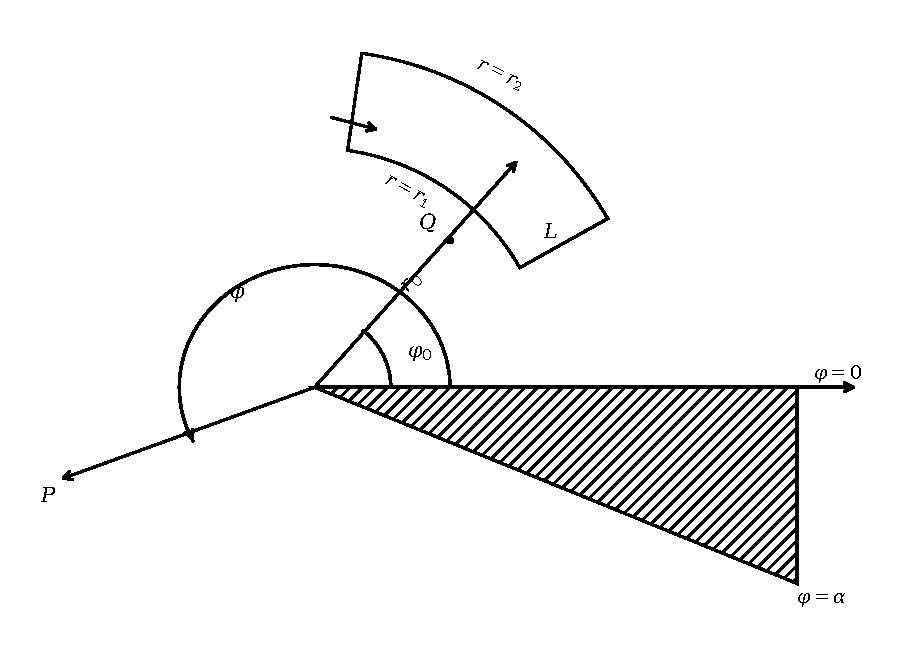
\includegraphics[width=.43\linewidth]{images/recreated/a-0020-fig.pdf}\par
Figure 1. The excitation of a wedge-shaped region by a linear source.\par
$Q$ -- source; $P$ -- the observation point;\par
$L$ -- the integration contour in Equation (1.10).\end{center}
\[\iint\delta(r-r_0,\phi-\phi_0)r\,dr\,d\phi=1\]
with integration over the neighborhood of the point $r_0,\phi_0$.

Here and henceforth, we will use the absolute system of units (the Gauss system), and we will assume the dependence on time is in the form $e^{-i\omega t}$.

In the first case, the ``electric'' vector potential $A_z^e$ satisfies the equation (see, for example, [4])
\[\Delta A_z^e+k^2A_z^e=-\frac{4\pi}{c}j_z^e\tag{1.03}\]
and the boundary condition
\[A_z^e=0\quad\text{with}\quad\phi=0\text{ and }\phi=\alpha.\tag{1.04}\]
\end{scanpage}
